\documentclass[border=6pt]{standalone}
\usepackage{amsmath,amssymb}
\usepackage{tikz}
\usetikzlibrary{arrows.meta,positioning,calc}

\newcommand{\ttl}{\scriptsize\bfseries}
\newcommand{\dsc}{\scriptsize}

\begin{document}
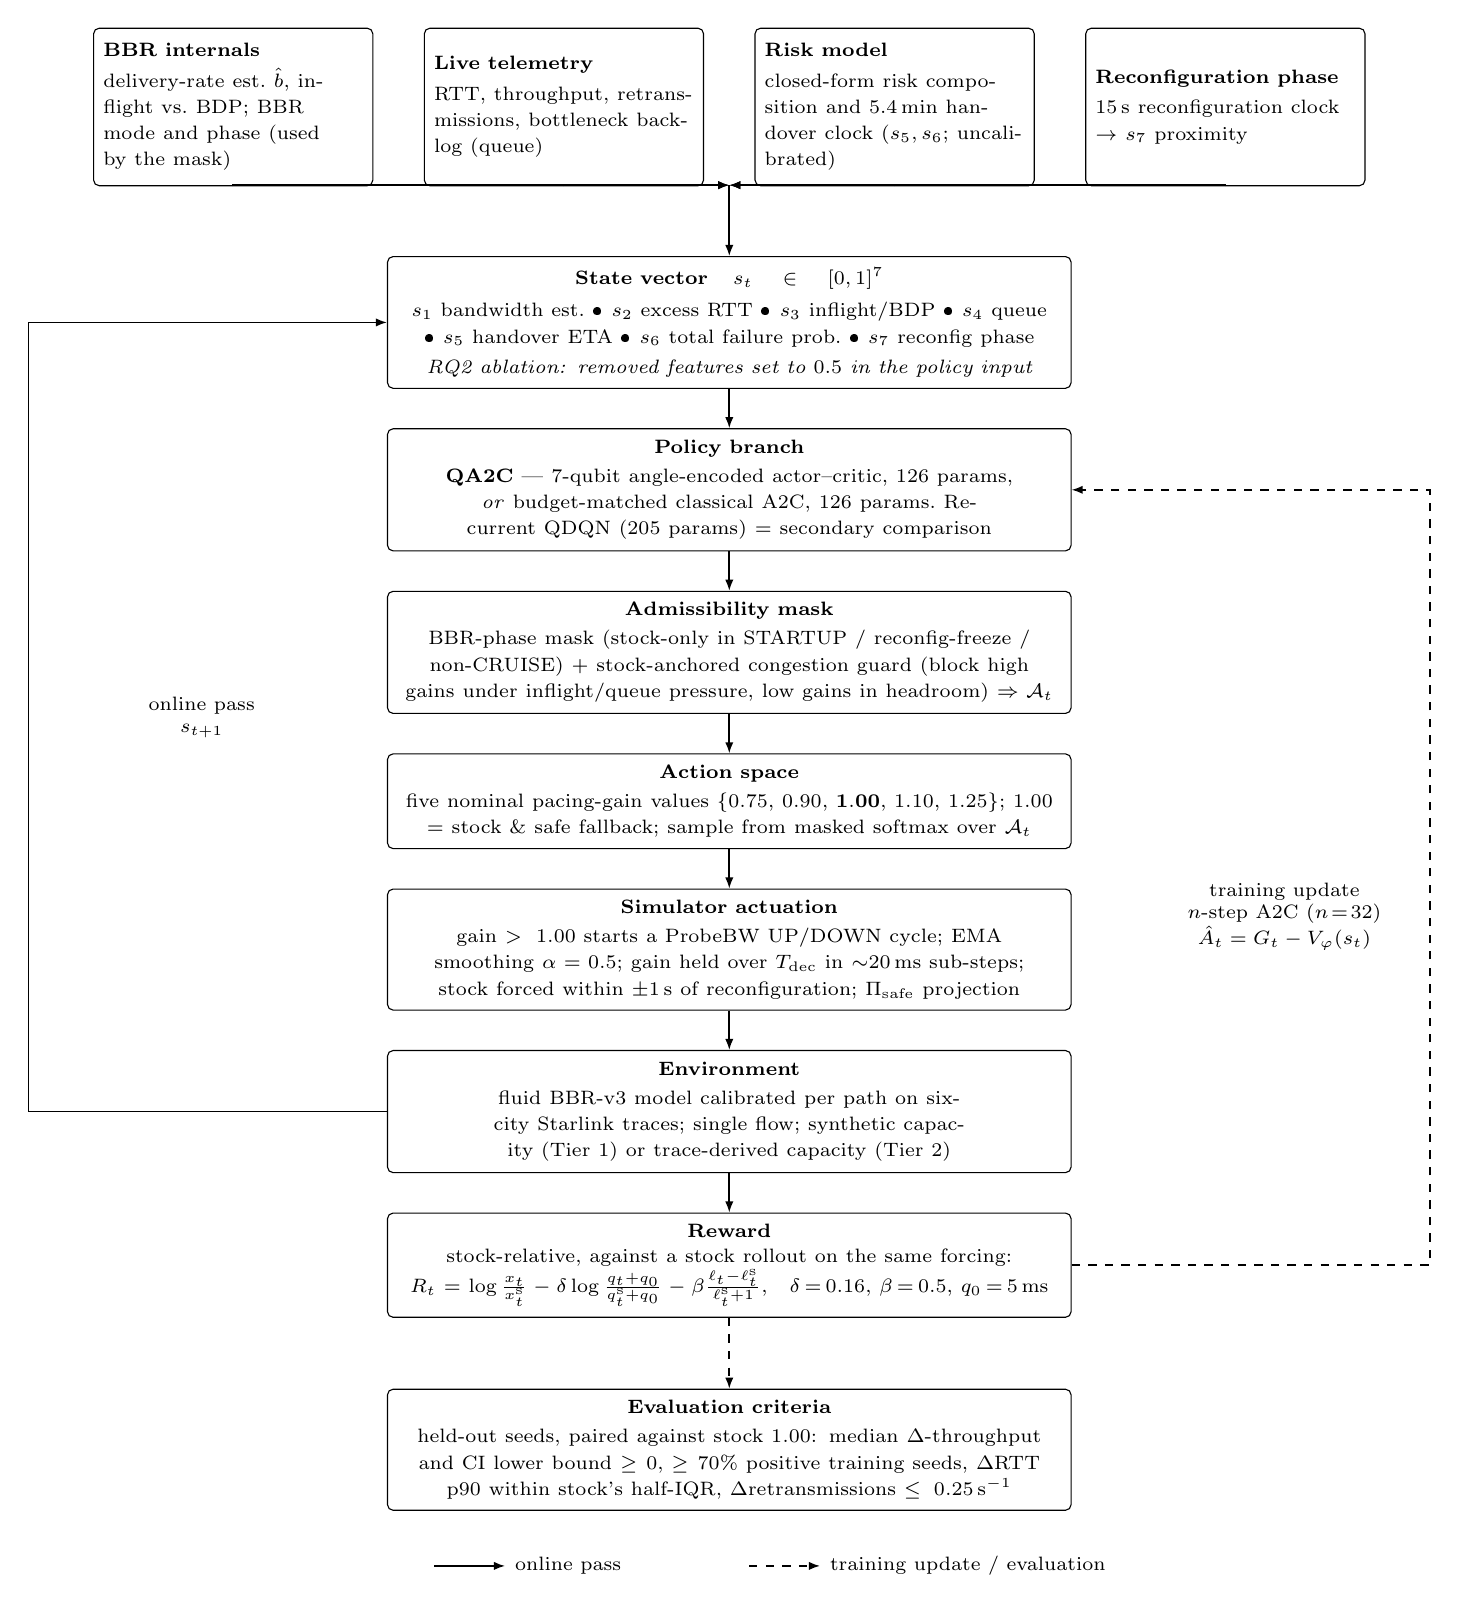
\begin{tikzpicture}[
  font=\footnotesize,
  bx/.style  = {draw, rounded corners=2pt, align=center, inner sep=4pt, text width=84mm},
  ibx/.style = {draw, rounded corners=2pt, align=left,  inner sep=3.5pt, text width=33mm,
                minimum height=20mm, anchor=north},
  ar/.style  = {-{Latex[length=4pt]}, semithick},
  dar/.style = {-{Latex[length=4pt]}, semithick, dashed}
]

% ---------- top: feature-provenance row ---------------------------------
\node[ibx] (in1) at (-6.3,0) {{\ttl BBR internals}\\[1.5pt]{\dsc delivery-rate est.\ $\hat b$, inflight vs.\ BDP; BBR mode and phase (used by the mask)}};
\node[ibx] (in2) at (-2.1,0) {{\ttl Live telemetry}\\[1.5pt]{\dsc RTT, throughput, retransmissions, bottleneck backlog (queue)}};
\node[ibx] (in3) at ( 2.1,0) {{\ttl Risk model}\\[1.5pt]{\dsc closed-form risk composition and 5.4\,min handover clock ($s_5,s_6$; uncalibrated)}};
\node[ibx] (in4) at ( 6.3,0) {{\ttl Reconfiguration phase}\\[1.5pt]{\dsc 15\,s reconfiguration clock $\rightarrow$ $s_7$ proximity}};

% ---------- vertical spine --------------------------------------------
\node[bx, anchor=north] (state) at (0,-2.9)
  {{\ttl State vector\quad $s_t\in[0,1]^{7}$}\\[2pt]
   {\dsc $s_1$ bandwidth est.\ \textbullet\ $s_2$ excess RTT \textbullet\ $s_3$ inflight/BDP \textbullet\ $s_4$ queue
    \textbullet\ $s_5$ handover ETA \textbullet\ $s_6$ total failure prob.\ \textbullet\ $s_7$ reconfig phase}\\[1.5pt]
   {\dsc\itshape RQ2 ablation: removed features set to $0.5$ in the policy input}};

\node[bx, below=5mm of state] (policy)
  {{\ttl Policy branch}\\[1pt]
   {\dsc \textbf{QA2C} --- 7-qubit angle-encoded actor--critic, 126 params, \emph{or}
    budget-matched classical A2C, 126 params.\ Recurrent QDQN (205 params) = secondary comparison}};

\node[bx, below=5mm of policy] (mask)
  {{\ttl Admissibility mask}\\[1pt]
   {\dsc BBR-phase mask (stock-only in STARTUP / reconfig-freeze / non-CRUISE) $+$
    stock-anchored congestion guard (block high gains under inflight/queue pressure,
    low gains in headroom) $\Rightarrow \mathcal{A}_t$}};

\node[bx, below=5mm of mask] (action)
  {{\ttl Action space}\\[1pt]
   {\dsc five nominal pacing-gain values $\{0.75,\,0.90,\,\mathbf{1.00},\,1.10,\,1.25\}$;
    $1.00$ = stock \& safe fallback; sample from masked softmax over $\mathcal{A}_t$}};

\node[bx, below=5mm of action] (act)
  {{\ttl Simulator actuation}\\[1pt]
   {\dsc gain $>1.00$ starts a ProbeBW UP/DOWN cycle; EMA smoothing $\alpha\!=\!0.5$; gain held over
    $T_{\text{dec}}$ in $\sim$20\,ms sub-steps; stock forced within $\pm1$\,s of reconfiguration; $\Pi_{\text{safe}}$ projection}};

\node[bx, below=5mm of act] (env)
  {{\ttl Environment}\\[1pt]
   {\dsc fluid BBR-v3 model calibrated per path on six-city Starlink traces; single flow;
    synthetic capacity (Tier~1) or trace-derived capacity (Tier~2)}};

\node[bx, below=5mm of env] (reward)
  {{\ttl Reward}\\[1pt]
   {\dsc stock-relative, against a stock rollout on the same forcing:\\
    $R_t=\log\frac{x_t}{x^{\mathrm{s}}_t}-\delta\log\frac{q_t+q_0}{q^{\mathrm{s}}_t+q_0}-\beta\frac{\ell_t-\ell^{\mathrm{s}}_t}{\ell^{\mathrm{s}}_t+1}$,\quad
    $\delta\!=\!0.16$, $\beta\!=\!0.5$, $q_0\!=\!5$\,ms}};

\node[bx, below=9mm of reward] (gate)
  {{\ttl Evaluation criteria}\\[1pt]
   {\dsc held-out seeds, paired against stock $1.00$: median $\Delta$-throughput and CI lower bound $\ge0$,
    $\ge70\%$ positive training seeds, $\Delta$RTT p90 within stock's half-IQR, $\Delta$retransmissions $\le0.25$\,s$^{-1}$}};

% ---------- provenance arrows into a bus ------------------------------
\coordinate (bus) at ($(state.north)+(0,9mm)$);
\foreach \n in {in1,in2,in3,in4}{\draw[ar] (\n.south) |- (bus);}
\draw[ar] (bus) -- (state.north);

% ---------- spine arrows -----------------------------------------------
\foreach \a/\b in {state/policy, policy/mask, mask/action, action/act, act/env, env/reward}{
  \draw[ar] (\a) -- (\b);}
\draw[dar] (reward) -- (gate);

% ---------- online feedback (left channel) ---------------------------
\coordinate (lmid) at ($(state.west)!0.5!(env.west)$);
\draw[ar] (env.west) -- (-8.9,0 |- env.west) |- (state.west);
\node[font=\scriptsize, align=center] at (-6.7,0 |- lmid) {online pass\\$s_{t+1}$};

% ---------- offline update (right channel) --------------------------
\coordinate (rmid) at ($(policy.east)!0.55!(reward.east)$);
\draw[dar] (reward.east) -- (8.9,0 |- reward.east) |- (policy.east);
\node[font=\scriptsize, align=center] at (7.05,0 |- rmid) {training update\\$n$-step A2C ($n\!=\!32$)\\$\hat A_t = G_t - V_\varphi(s_t)$};

% ---------- legend --------------------------------------------------
\draw[ar]  ($(gate.south west)+(6mm,-7mm)$) -- ++(9mm,0) node[right,font=\scriptsize] {online pass};
\draw[dar] ($(gate.south west)+(46mm,-7mm)$) -- ++(9mm,0) node[right,font=\scriptsize] {training update / evaluation};

\end{tikzpicture}
\end{document}
